% ======== 卷首上（8行21字）========
\chapter*{欽定儀象考成卷首上}
\begin{正文}
\end{正文}\clearpage
\thispagestyle{empty}\noindent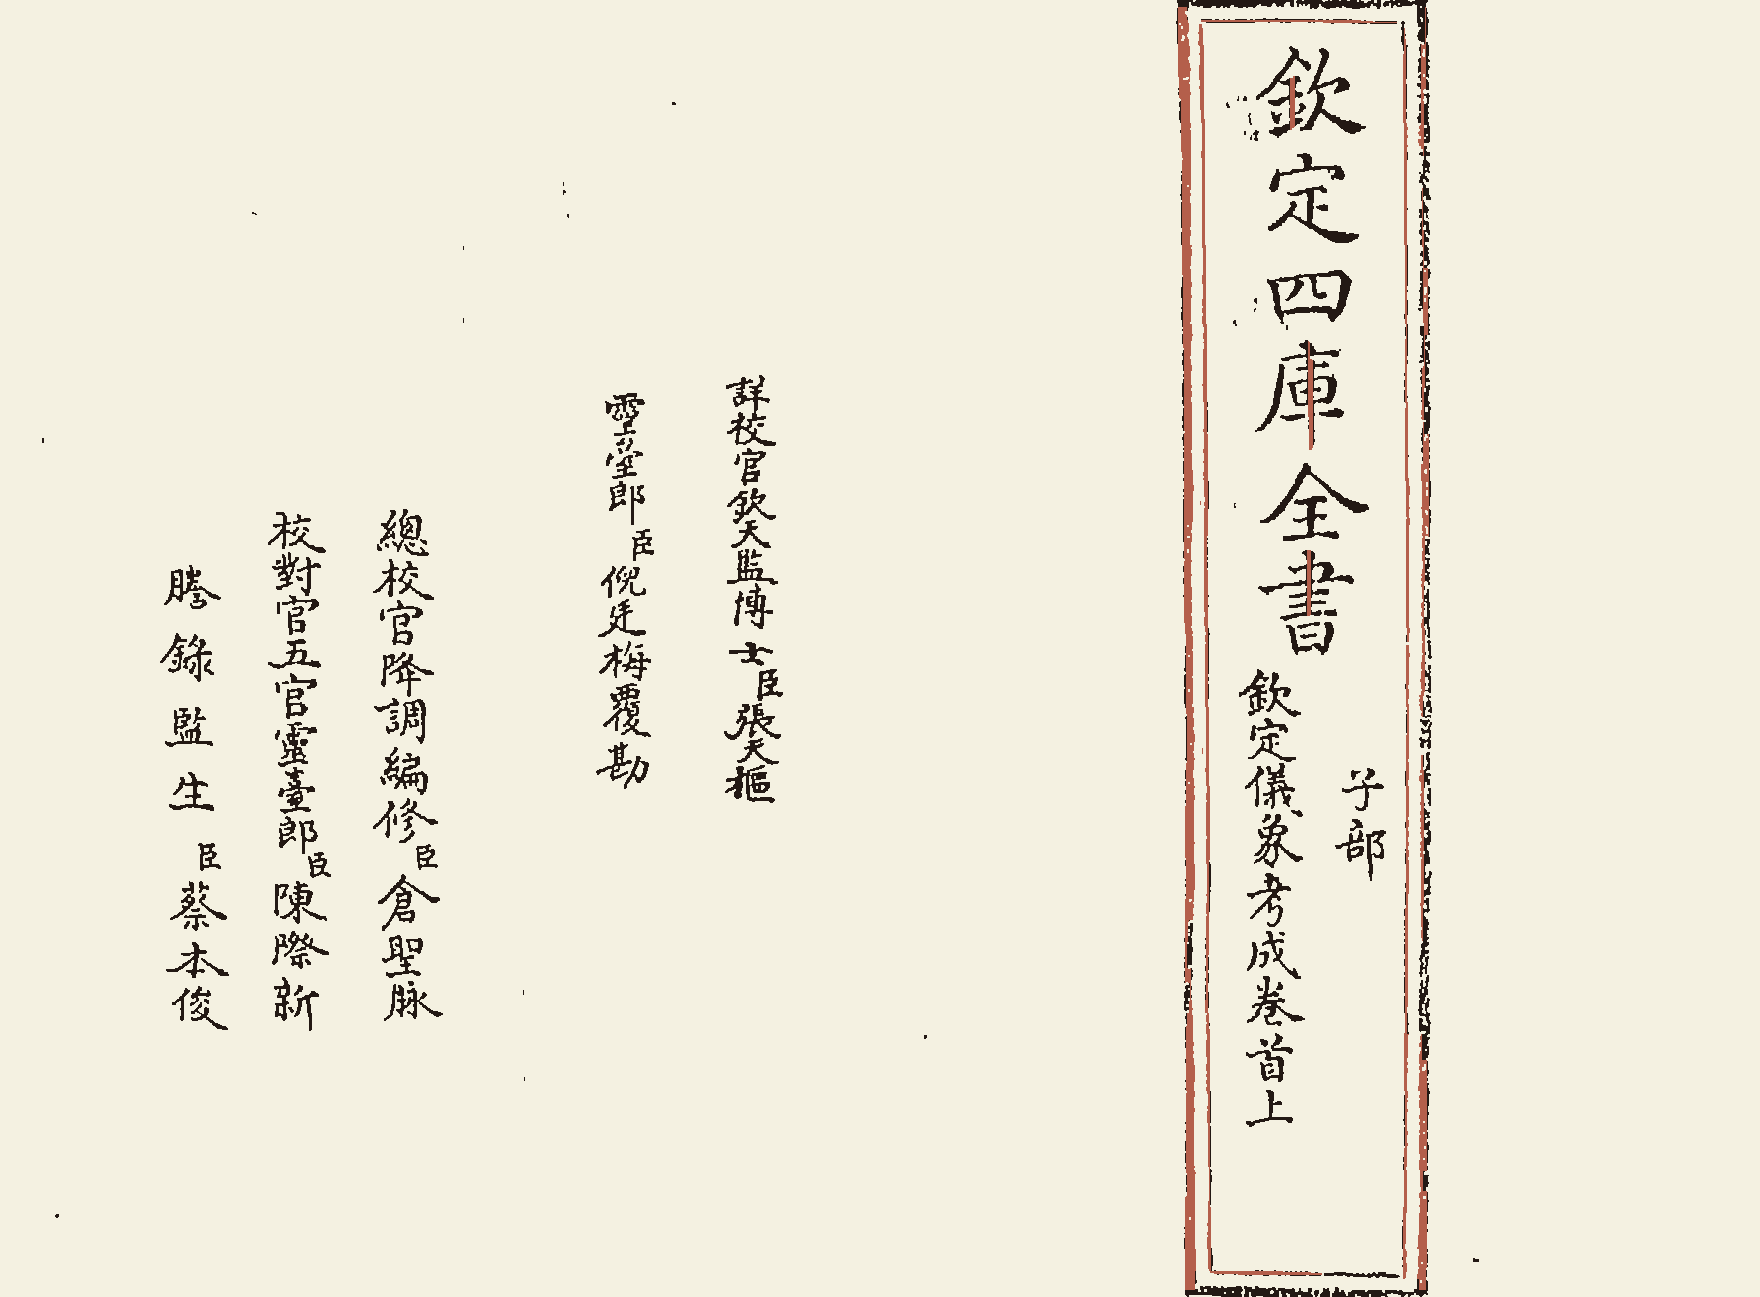
\includegraphics[width=\paperwidth,height=\paperheight,keepaspectratio]{img/0092.png}\clearpage
\begin{正文}
% ---- 册793 葉93 ----
\SetPageNumber{1}
欽定四庫全書\换行
欽定儀象考成卷首上\换行
御製璣衡撫辰儀説卷上\换行
　　儀制\换行
　　製法\换行
\char"200B\relax\换行
\char"200B\relax\换行
\char"200B\relax\换行
\char"200B\relax\换行
\char"200B\relax\换行
\char"200B\relax\换行
\char"200B\relax\换行
\char"200B\relax\换行
\char"200B\relax\换行
\char"200B\relax\换行
\char"200B\relax
\par
% ---- 册793 葉96 ----
御製璣衡撫辰儀説卷上之一\换行
　儀制\换行
　　全儀\换行
　　子午圏\换行
　　天常赤道\换行
　　赤極經圏\换行
　　遊旋赤道\换行
　　四遊圏\换行
　　指時度表\换行
　　借弧指時度表\换行
　　指緯度表\换行
　　立表\换行
　　平行立表\换行
　　平行借弧表\换行
　　綰經度表\换行
　　綰時度表
\par
% ---- 册793 葉97 ----
　　平行線測經度表\换行
\char"200B\relax\换行
\char"200B\relax\换行
\char"200B\relax\换行
\char"200B\relax\换行
\char"200B\relax\换行
\char"200B\relax\换行
\char"200B\relax\换行
\char"200B\relax\换行
\char"200B\relax\换行
\char"200B\relax\换行
\char"200B\relax\换行
\char"200B\relax\换行
\char"200B\relax\换行
\char"200B\relax\换行
\char"200B\relax
\par
\end{正文}\clearpage
\嵌图{153.00pt}{215.88pt}{395.02pt}{576.95pt}{img/0100.png}
\begin{正文}
% ---- 册793 葉100 ----
\SetPageNumber{4}
\插图页
\char"200B\relax\换行
\char"200B\relax\换行
\char"200B\relax\换行
\char"200B\relax\换行
\char"200B\relax\换行
\char"200B\relax\换行
\char"200B\relax\换行
\char"200B\relax\换行
\恢复丝栏
　　虞書舜典在璿璣玉衡以齊七政孔穎逹疏曰璣\换行
　　衡者王者正天文之器漢世以來謂之渾天儀者\换行
　　是也馬融云渾天儀可旋轉故曰璣衡其横簫所\换行
　　以視星宿也蔡邕云衡長八尺孔徑一寸下端望\换行
　　之以視星辰盖懸璣以象天而衡望之轉璣窺衡\换行
　　以知星宿是其説也上天之體不可得知測天之\换行
　　事見於經者惟此璿璣玉衡一事而已楊子法言\换行
　　云或問渾天曰落下閎營之鮮于妄人度之耿中
\par
% ---- 册793 葉101 ----
　　丞象之幾乎幾乎莫之能違也閎與妄人武帝時\换行
　　人宣帝時司農中丞耿夀昌始鑄銅為之象史官\换行
　　施用焉江南宋元嘉年太史丞錢樂\双列{\右小列{陳氏師凱曰}\左小列{錢樂本名樂}}\换行
　　\双列{\右小列{之孔疏}\左小列{脱之字}}鑄銅作渾天儀傳於齊梁周平江陵遷於\换行
　　長安尚書蔡註曰宋錢樂鑄銅作渾天儀衡長八\换行
　　尺孔徑一寸璣徑八尺圓周二丈五尺强轉而望\换行
　　之以知日月星辰之所在即璿璣玉衡之遺法也\换行
　　厯代以來其法漸密本朝因之為儀三重其在外\换行
　　者曰六合儀平置黒單環上刻十二辰八干四隅\换行
　　在地之位以凖地面而定四方側立黒雙環背刻\换行
　　去極度數以中分天脊直跨地平使其半入地下\换行
　　而結於其子午以為天經斜倚赤單環背刻赤道\换行
　　度數以平分天腹横繞天經亦使半出地上半入\换行
　　地下而結於其卯酉以為天緯三環表裏相結不\换行
　　動其天經之環則南北二極皆為圓軸虚中而内\换行
　　向以挈三辰四遊之環以其上下四方於是可考
\par
% ---- 册793 葉104 ----
　　故曰六合次其内曰三辰儀側立黒雙環亦刻去\换行
　　極度數外貫天經之軸内挈黄赤二道其赤道則\换行
　　為赤單環外依天緯亦刻宿度而結於黒雙環之\换行
　　卯酉其黄道則為黄單環亦刻宿度而又斜倚於\换行
　　赤道之腹以交結於卯酉而半入其内以為春分\换行
　　後之日軌半出其外以為秋分後之日軌又為白\换行
　　單環以承其交使不傾墊以其日月星辰於是可\换行
　　考故曰三辰其最在内者曰四遊儀亦為黒雙環\换行
　　如三辰儀之制以貫天經之軸其環之内則兩面\换行
　　當中各施直距外指兩軸而當其要中之内面又\换行
　　為小窽以受玉衡要中之小軸使衡既得隨環東\换行
　　西運轉又可隨處南北低昻以待占𠉀者之仰窺\换行
　　焉以其東西南北無不周徧故曰四遊此其法之\换行
　　大畧也今考前史漢初落下閎造渾天儀本無黄\换行
　　道或云賈逵所加或云李淳風所加或云一行所\换行
　　加而宋錢樂之渾儀之制雖有黄道並無黄道經
\par
% ---- 册793 葉105 ----
　　圈其四遊圈亦不貫於黄極則亦未盡黄道之用\换行
　　元郭守敬作簡儀乃分渾儀而變其制别設立運\换行
　　圏以測地平經緯度而不設黄道圏盖黄道與黄\换行
　　極經圏成經緯設黄道又設經圏則圏多而不便\换行
　　於測𠉀故不用黄道而專用赤道圈明正統三年\换行
　　　鑄銅渾儀簡儀於北京即宋元遺法也我\换行
　　朝康熙八年\换行
\抬头[1]聖祖仁皇帝命監臣南懐仁新製六儀赤道黄道分為二\换行
　　器皆不用地平圏而地平象限天體諸儀則地平\换行
　　之經緯與黄赤之錯綜皆已畢具康熙五十二年\换行
　　　又\换行
\抬头[1]命監臣紀利安製地平經緯儀合地平象限二儀而為一\换行
　　　其用尤便制作之妙於斯極矣我\换行
　皇上敬\换行
天法\换行
祖齊政勤民
\par
% ---- 册793 葉108 ----
親蒞靈臺徧觀儀象以渾天制最近古而時度信宜從\换行
　　今觀其㑹通斯成鉅典於是用今之數目合古之\换行
　　型模\换行
御製璣衡撫辰儀用裨測𠉀誠唐虞之遺意昭代之新\换行
　　規也儀制三重其在外者即古之六合儀而不用\换行
　　地平圏其正立雙環為子午圏兩面皆刻周天三\换行
　　百六十度自南北極起初度至中要九十度是為\换行
　　天經斜倚單環為天常赤道圏兩面皆刻周日十\换行
　　二時以子正午正當子午雙環中空之半而結於\换行
　　其中要是為天緯其南北二極皆設圓軸軸本實\换行
　　於子午雙環中空之間而軸内向以貫内二重之\换行
　　環其下承以雲座仰面正中開雙槽以受雙環東\换行
　　面正中開雲窩以受垂球下面置十字架施螺旋\换行
　　以取平架之東西兩端各植龍柱龍口銜珠開孔\换行
　　以承天常赤道卯酉之兩軸依觀象臺測定南北\换行
　　正線将座架安定則平面之四方正又依京師北
\par
% ---- 册793 葉109 ----
　　極出地三十九度五十五分自北極而上五十度\换行
　　五分即上應天頂自南極而下五十度五分即下\换行
　　對地心而應天頂之衝於天頂施小釘懸垂線而\换行
　　垂適當地心又適切於雙環之面不即不離則上\换行
　　下正立面之四方亦正而地平已在其中故不用\换行
　　地平圏也次其内即古之三辰儀而不用黄道圏\换行
　　其貫於二極之雙環為赤極經圏兩極各設軸孔\换行
　　以受天經之軸兩面皆刻周天三百六十度結於\换行
　　赤極經圏之中要與天常赤道平運者為遊旋赤\换行
　　道圈兩面皆刻周天三百六十度與天之赤道旋\换行
　　轉相應自經圏之南極作兩象限弧以承之使不\换行
　　傾墊測得三辰之赤道經緯度則黄道經緯可推\换行
　　且黄道與赤道之相距古逺今近縱或日久有差\换行
　　而儀器無庸改制故不用黄道圏也其在内者即\换行
　　古之四遊儀貫於二極之雙環為四遊圏兩面皆\换行
　　刻三百六十度定於遊圏之兩極者為直距綰於
\par
% ---- 册793 葉112 ----
　　直距之中心者為窺衡遊圏中要設直表以指經\换行
　　度及時窺衡右旁設直表以指緯度此古今所同\换行
　　無容置議者也是故體制倣乎渾天之舊而時度\换行
　　尤為整齊運量同於赤道新儀而重環更能合應\换行
　　至於借表窺測則上下左右無不宜焉夫羲和遺\换行
　　制不可考已漢世以來或作而不傳或傳而不久\换行
　　盖制器尚象若斯之難也而稽古宜今至我\换行
　朝乃臻盡善易繫傳云備物致用立成器以為天下\换行
　　利莫大乎聖人詎不信乎\换行
\char"200B\relax\换行
\char"200B\relax\换行
\char"200B\relax\换行
\char"200B\relax\换行
\char"200B\relax\换行
\char"200B\relax\换行
\char"200B\relax
\par
\end{正文}\clearpage
\嵌图{154.79pt}{220.57pt}{393.23pt}{572.26pt}{img/0118.png}
\begin{正文}
% ---- 册793 葉118 ----
\SetPageNumber{11}
\插图页
\char"200B\relax\换行
\char"200B\relax\换行
\char"200B\relax\换行
\char"200B\relax\换行
\char"200B\relax\换行
\char"200B\relax\换行
\char"200B\relax\换行
\char"200B\relax\换行
\恢复丝栏
子午圈所以正南北也天之南北定於兩極必先測定\换行
南北正線而後安置子午圈則子午圈即為南北之正\换行
線南北正而後日軌之髙下時刻之早晚中星之偏度\换行
可得而稽也其制雙環外徑六尺三寸内徑五尺六寸\换行
六分環面濶三寸二分厚九分中空一寸雙環之間四\换行
隅各施銅枕合而固之其中空之半為子午正線兩面\换行
各畫三百六十度每度六十分自南北極起初度至中\换行
要九十度古曰天經環西法舊曰緯圈盖織絲以直者
\par
% ---- 册793 葉122 ----
為經横者為緯古以其圈直立故曰經西法以其為横\换行
線所界之度故曰緯今按圈直而度横則其圈宜曰經\换行
圈而其度乃為緯度周禮賈公彦疏所謂南北之道謂\换行
之經元儒陳氏師凱所謂自北數向南去如機上數緯\换行
絲是也自兩極起初度者北極出地南極入地其度數\换行
皆自兩極起算也中要九十度者赤道為帯天之紘距\换行
兩極各一象限也南北極各設鋼軸軸本扁方長三寸\换行
濶二寸二分厚一寸實於隻環之間以鋼螺旋結之軸\换行
長六寸徑八分正當雙環中空之半内向以貫三辰四\换行
遊之環所以象天樞也\换行
\char"200B\relax\换行
\char"200B\relax\换行
\char"200B\relax\换行
\char"200B\relax\换行
\char"200B\relax\换行
\char"200B\relax
\par
\end{正文}\clearpage
\嵌图{148.32pt}{219.14pt}{399.70pt}{573.69pt}{img/0126.png}
\begin{正文}
% ---- 册793 葉126 ----
\SetPageNumber{13}
\插图页
\char"200B\relax\换行
\char"200B\relax\换行
\char"200B\relax\换行
\char"200B\relax\换行
\char"200B\relax\换行
\char"200B\relax\换行
\char"200B\relax\换行
\char"200B\relax\换行
\恢复丝栏
天常赤道所以正時刻也天左旋一日一周南北極持\换行
其兩端而赤道為其横帯以其常定不動故曰天常日\换行
循黄道右旋而其隨天西轉則係赤道之度日行臨於\换行
赤道之某位即為某時故時刻由赤道而正也其制單\换行
環外徑六尺一寸二分内徑五尺六寸四分環面濶二\换行
寸四分厚一寸四分平分其厚為赤道之中線兩面各\换行
畫周日十二時每時初正各四刻每刻十五分每一時\换行
當天之三十度每四刻當天之十五度每一分當天之
\par
% ---- 册793 葉130 ----
十五分以其子正午正線當子午雙環中空之半而結\换行
於其中要使其赤道中線適當子午圏之九十度兩圈\换行
相結成十字直角古曰天緯環西法舊曰赤道經圈盖\换行
古以其圈横運故曰緯西法以其為直線所界之度故\换行
曰經今按圈横而度直則其圈宜曰緯圈而其度乃為\换行
經度周禮賈公彦疏所謂東西之道謂之緯陳氏師凱\换行
所謂自東數向西去如機上數經絲是也上面午正時\换行
刻線結於子午圈之正北卯正居西酉正居東謂日影\换行
對照之時下面則子正居北午正居南卯正居東酉正\换行
居西為日行所臨之正位也\换行
\char"200B\relax\换行
\char"200B\relax\换行
\char"200B\relax\换行
\char"200B\relax\换行
\char"200B\relax\换行
\char"200B\relax
\par
\end{正文}\clearpage
\嵌图{153.38pt}{219.23pt}{394.64pt}{573.60pt}{img/0134.png}
\begin{正文}
% ---- 册793 葉134 ----
\SetPageNumber{15}
\插图页
\char"200B\relax\换行
\char"200B\relax\换行
\char"200B\relax\换行
\char"200B\relax\换行
\char"200B\relax\换行
\char"200B\relax\换行
\char"200B\relax\换行
\char"200B\relax\换行
\恢复丝栏
赤極經圏所以帯赤道也亦曰過極圏制如子午雙環\换行
在内而差小外徑五尺五寸六分内徑五尺一寸二分\换行
環面濶二寸二分厚八分中空一寸二分兩面皆畫三\换行
百六十度每度六十分一面自兩極起初度至赤道九\换行
十度以應天經一面自赤道起初度至兩極九十度以\换行
應赤緯南北極各設軸孔用扁方銅長三寸濶與環面\换行
等厚與雙環中空等中心開圓孔以受天經之軸其孔\换行
徑適容軸徑使旋轉不致動摇孔之兩面各施鋼片厚
\par
% ---- 册793 葉138 ----
四分使孔徑不致磨損兩軸孔之中徑適當雙環中空\换行
之半與兩極徑線參直以鋼螺旋結之環外南北極之\换行
兩端各施扁圓鋼子厚五分與内外兩雙環之分縫等\换行
貫於天經之軸使赤極經圈之中要九十度線適與子\换行
午圈之九十度相凖則内外兩圈上下四方俱合為一\换行
線而縱横經緯自宜悉協矣\换行
\char"200B\relax\换行
\char"200B\relax\换行
\char"200B\relax\换行
\char"200B\relax\换行
\char"200B\relax\换行
\char"200B\relax\换行
\char"200B\relax\换行
\char"200B\relax\换行
\char"200B\relax\换行
\char"200B\relax
\par
\end{正文}\clearpage
\嵌图{157.41pt}{218.38pt}{390.61pt}{574.45pt}{img/0142.png}
\begin{正文}
% ---- 册793 葉142 ----
\SetPageNumber{17}
\插图页
\char"200B\relax\换行
\char"200B\relax\换行
\char"200B\relax\换行
\char"200B\relax\换行
\char"200B\relax\换行
\char"200B\relax\换行
\char"200B\relax\换行
\char"200B\relax\换行
\恢复丝栏
遊旋赤道所以象天之運行而紀其赤道經度也制如\换行
天常赤道在内而差小外徑五尺五寸六分内徑五尺\换行
一寸二分環面濶二寸二分厚一寸二分平分其厚為\换行
赤道之中線兩面各畫周天三百六十度上面分為十\换行
二宫每宫三十度每度六十分下面自丑宫起初度右\换行
旋三百六十度以其丑宫未宫初度之線當赤經雙環\换行
中空之半而結於其中要使其赤道中線適當經圈之\换行
九十度兩圈相結成十字直角與天之赤道旋轉相應
\par
% ---- 册793 葉146 ----
又於經圏南極之兩旁設象限弧承於遊旋赤道辰宫\换行
戌宫之下以螺旋結之使不傾墊有天常赤道之不動\换行
者以定時又有遊旋赤道之常動者以紀度則赤道之\换行
逐宫逐度皆能周行於十二時而三辰之所躔與兩曜\换行
之相距皆可得而稽矣\换行
\char"200B\relax\换行
\char"200B\relax\换行
\char"200B\relax\换行
\char"200B\relax\换行
\char"200B\relax\换行
\char"200B\relax\换行
\char"200B\relax\换行
\char"200B\relax\换行
\char"200B\relax\换行
\char"200B\relax\换行
\char"200B\relax
\par
\end{正文}\clearpage
\嵌图{152.17pt}{219.82pt}{395.85pt}{573.01pt}{img/0150.png}
\begin{正文}
% ---- 册793 葉150 ----
\SetPageNumber{19}
\插图页
\char"200B\relax\换行
\char"200B\relax\换行
\char"200B\relax\换行
\char"200B\relax\换行
\char"200B\relax\换行
\char"200B\relax\换行
\char"200B\relax\换行
\char"200B\relax\换行
\恢复丝栏
四遊圈所以測三辰之赤道經緯度也制如赤經雙環\换行
在内而差小外徑五尺内徑四尺六寸八分環面濶一\换行
寸六分厚七分中空一寸四分盖三重雙環之外面皆\换行
相平而内重則漸薄中空則漸大取其輕重適宜亦便\换行
於設窺衡也兩面各畫三百六十度一面自北極起初\换行
度至南極一百八十度為去極度一面自赤道起初度\换行
至兩極各九十度為距緯度南北極各設軸孔以受夭\换行
經之軸與過極圈同環外南北極之兩端各施扁圓鋼
\par
% ---- 册793 葉152 ----
子厚六分與赤經四遊兩環之分縫等貫於天經之軸\换行
其下半周之中要安直表以指經度及時刻兩面對南\换行
北極各安直距如圓之通徑濶一寸六分厚七分中空\换行
一寸四分直距之二面對環之兩極作直徑線對環之\换行
九十度作横徑線十字相交中心開圓孔施螺旋小鋼\换行
軸而圓其末以綰窺衡窺衡長四尺七寸二分方一寸\换行
二分中空一寸上下兩端施方銅盖厚五分内三分方\换行
一寸入於管中外二分方一寸二分齊於管面中心開\换行
圓孔上端孔心留十字線以便測視管之四面亦各取\换行
中線上面安立表下端右面安指緯度表左右兩面之\换行
中心各開圓孔使直距中要小軸之末入其中以綰之\换行
則窺衡乃能南北低昂而隨雙環東西運轉焉窺衡連\换行
盖長四尺七寸六分比四遊環内徑長八分兩端各施\换行
鋼篐厚一分中要孔外施鋼眼錢亦厚一分使其左右\换行
適切於中空之内面上下兩端入於雙環内徑各四分\换行
則上下低昂自無偏側而所測經緯度必皆密合矣
\par
\end{正文}\clearpage
\嵌图{153.29pt}{217.38pt}{394.73pt}{575.45pt}{img/0153.png}
\begin{正文}
% ---- 册793 葉153 ----
\SetPageNumber{21}
\插图页
\char"200B\relax\换行
\char"200B\relax\换行
\char"200B\relax\换行
\char"200B\relax\换行
\char"200B\relax\换行
\char"200B\relax\换行
\char"200B\relax\换行
\char"200B\relax\换行
\恢复丝栏
指時度表通長七寸三分本長一寸六分形如方筒入\换行
於四遊雙環中空之間濶一寸四分與四遊環之中空\换行
等平分其濶即當窺衡之中線筒中施左右螺旋以充\换行
塞於中空之内使表不動移横帶長三寸二分濶五分\换行
兩端各鉤囬二分扣於環面之外表長五寸二分濶一\换行
寸其指時度之邊線對方筒之正中亦即窺衡之正中\换行
下端二寸四分厚三分切於遊旋赤道之面以指度分\换行
上端二寸八分厚二分切於天常赤道之面以指時刻
\par
% ---- 册793 葉156 ----
也\换行
\char"200B\relax\换行
\char"200B\relax\换行
\char"200B\relax\换行
\char"200B\relax\换行
\char"200B\relax\换行
\char"200B\relax\换行
\char"200B\relax\换行
\char"200B\relax\换行
\char"200B\relax\换行
\char"200B\relax\换行
\char"200B\relax\换行
\char"200B\relax\换行
\char"200B\relax\换行
\char"200B\relax\换行
\char"200B\relax
\par
\end{正文}\clearpage
\嵌图{151.20pt}{217.28pt}{396.82pt}{575.55pt}{img/0157.png}
\begin{正文}
% ---- 册793 葉157 ----
\SetPageNumber{23}
\插图页
\char"200B\relax\换行
\char"200B\relax\换行
\char"200B\relax\换行
\char"200B\relax\换行
\char"200B\relax\换行
\char"200B\relax\换行
\char"200B\relax\换行
\char"200B\relax\换行
\恢复丝栏
借弧指時度表其本方筒及横帶長濶並與前指時度\换行
表同横帶之下自左向右立安弧背一道長九寸三分\换行
濶一寸二分厚一分六釐弧背之末平安指時度表除\换行
弧背之厚長五寸二分濶一寸計自表本方筒之中線\换行
至指時度表之内邊長六寸七分當遊旋赤道之十五\换行
度當天常赤道之一小時測量時指時度表或為子午\换行
圏所礙則用此表視其所指之時度加四刻即為所測\换行
之時減十五度即為所測之度盖借弧指時度表在窺
\par
% ---- 册793 葉160 ----
衡之右所指雖視乎借表而所測則定於窺衡天常之\换行
時刻左旋故加三辰之度分右旋故減則用借弧指時\换行
度表察之與用指時度表等也\换行
\char"200B\relax\换行
\char"200B\relax\换行
\char"200B\relax\换行
\char"200B\relax\换行
\char"200B\relax\换行
\char"200B\relax\换行
\char"200B\relax\换行
\char"200B\relax\换行
\char"200B\relax\换行
\char"200B\relax\换行
\char"200B\relax\换行
\char"200B\relax\换行
\char"200B\relax
\par
\end{正文}\clearpage
\嵌图{151.20pt}{220.43pt}{396.82pt}{572.40pt}{img/0161.png}
\begin{正文}
% ---- 册793 葉161 ----
\SetPageNumber{25}
\插图页
\char"200B\relax\换行
\char"200B\relax\换行
\char"200B\relax\换行
\char"200B\relax\换行
\char"200B\relax\换行
\char"200B\relax\换行
\char"200B\relax\换行
\char"200B\relax\换行
\恢复丝栏
指緯度表其形兩曲安於窺衡下端之右面底長三寸\换行
濶九分平分其濶為中線對衡面中線以螺旋結之曲\换行
横七分與四遊環之厚等又曲長一寸七分切於四遊\换行
環之外面從中線減濶之半所以指緯度也\换行
\char"200B\relax\换行
\char"200B\relax\换行
\char"200B\relax\换行
\char"200B\relax
\par
\end{正文}\clearpage
\嵌图{153.29pt}{219.54pt}{394.73pt}{573.29pt}{img/0164.png}
\begin{正文}
% ---- 册793 葉164 ----
\SetPageNumber{26}
\插图页
\char"200B\relax\换行
\char"200B\relax\换行
\char"200B\relax\换行
\char"200B\relax\换行
\char"200B\relax\换行
\char"200B\relax\换行
\char"200B\relax\换行
\char"200B\relax\换行
\恢复丝栏
立表二座形直底平表髙底長各三寸二分濶九分厚\换行
一分平分其濶為中線表直立於底長之半與底面成\换行
直角距底面一寸一表向上開長方孔長一寸中留直\换行
線又上五分開圓孔徑四分中留十字線安於窺衡之\换行
上端一表依前度下開直縫上開小圓孔安於窺衡之\换行
下端各對衡面中線以螺旋結之測量時窺衡或為赤\换行
道及銅枕所礙則用此表盖兩表之孔心中線距衡面\换行
皆相等又與衡面之中線參直則用立表測之與用窺
\par
% ---- 册793 葉165 ----
衡等也\换行
\char"200B\relax\换行
\char"200B\relax\换行
\char"200B\relax\换行
\char"200B\relax\换行
\char"200B\relax\换行
\char"200B\relax\换行
\char"200B\relax\换行
\char"200B\relax\换行
\char"200B\relax\换行
\char"200B\relax\换行
\char"200B\relax\换行
\char"200B\relax\换行
\char"200B\relax\换行
\char"200B\relax\换行
\char"200B\relax
\par
\end{正文}\clearpage
\嵌图{153.00pt}{217.70pt}{395.02pt}{575.13pt}{img/0168.png}
\begin{正文}
% ---- 册793 葉168 ----
\SetPageNumber{28}
\插图页
\char"200B\relax\换行
\char"200B\relax\换行
\char"200B\relax\换行
\char"200B\relax\换行
\char"200B\relax\换行
\char"200B\relax\换行
\char"200B\relax\换行
\char"200B\relax\换行
\恢复丝栏
平行立表二座形曲底平底盤長四寸濶一寸二分厚\换行
一分中空長三寸二分濶九分與立表底盤之長濶等\换行
表曲如勾股股直如立表髙三寸二分濶九分勾横連\换行
於股末長五寸濶九分横植於底盤之末底盤中空冒\换行
於立表底盤之外以掐表固之測量時窺衡立表或為\换行
子午圏及龍柱所礙則用此表盖平行立表曲如勾股\换行
而與立表平行則用平行立表測之與用立表等亦與\换行
用窺衡等也
\par
\end{正文}\clearpage
\嵌图{153.00pt}{223.19pt}{395.02pt}{569.64pt}{img/0169.png}
\begin{正文}
% ---- 册793 葉169 ----
\SetPageNumber{29}
\插图页
\char"200B\relax\换行
\char"200B\relax\换行
\char"200B\relax\换行
\char"200B\relax\换行
\char"200B\relax\换行
\char"200B\relax\换行
\char"200B\relax\换行
\char"200B\relax\换行
\恢复丝栏
平行借弧表制如平行立表而倒正異盖四遊窺衡東\换行
西為子午圏及龍柱所礙南北為赤道及銅枕所礙則\换行
用平行立表猶是窺衡所能及而管孔被遮故其表平\换行
行正立即可見若近北極之星則東西既礙於子午圏\换行
南北又礙於極軸窺衡不能及自上測之不能及北極\换行
之南六度餘自下測之不能及北極之北六度餘故借\换行
十度作平行借弧表一表上植一表下垂則窺衡未及\换行
北極十度而窺孔之視線已與北極參直其法以半徑
\par
% ---- 册793 葉172 ----
一千萬為一率十度之正切線一百七十六萬三千二\换行
百七十為二率表之横勾距窺衡中心二尺三寸三分\换行
為三率求得四率四寸一分零八毫為表髙之中數\双列{\右小列{自}\左小列{窺}}\换行
\双列{\右小列{衡中線至直}\左小列{距中線之數}}上端之表立植於衡面則中數即表髙\双列{\右小列{中}\左小列{數}}\换行
\双列{\右小列{減衡方之半六分加表端距窺孔中心}\左小列{六分為表端至表本之髙仍與中數等}}下端之表自衡\换行
面下垂則於中數加衡方之半六分表端距窺孔中心\换行
六分又加平行横勾之濶九分得六寸二分零八毫為\换行
表之髙距表端下六分開圓孔又下五分開長方孔皆\换行
與立表制同凡測近北極之星測得距赤道北若干加\换行
十度即得星距赤道北之緯度若測赤道南之星亦可\换行
用此表但測得距赤道南若干減十度即得星距赤道\换行
南之緯度也\换行
\char"200B\relax\换行
\char"200B\relax\换行
\char"200B\relax\换行
\char"200B\relax
\par
\end{正文}\clearpage
\嵌图{155.09pt}{220.28pt}{392.93pt}{572.55pt}{img/0173.png}
\begin{正文}
% ---- 册793 葉173 ----
\SetPageNumber{31}
\插图页
\char"200B\relax\换行
\char"200B\relax\换行
\char"200B\relax\换行
\char"200B\relax\换行
\char"200B\relax\换行
\char"200B\relax\换行
\char"200B\relax\换行
\char"200B\relax\换行
\恢复丝栏
綰經度表通長四寸濶一寸四分平分其濶即當窺衡\换行
之中線其本方筒長一寸六分髙一寸八分入於四遊\换行
雙環之間以左右螺旋固之其末上下二面以夾遊旋\换行
赤道上面濶七分減本之半與窺衡中線參直下面以\换行
螺旋固之所以綰定遊旋赤道之經度於四遊圈也\换行
\char"200B\relax\换行
\char"200B\relax\换行
\char"200B\relax
\par
\end{正文}\clearpage
\嵌图{153.29pt}{222.42pt}{394.73pt}{570.41pt}{img/0176.png}
\begin{正文}
% ---- 册793 葉176 ----
\SetPageNumber{32}
\插图页
\char"200B\relax\换行
\char"200B\relax\换行
\char"200B\relax\换行
\char"200B\relax\换行
\char"200B\relax\换行
\char"200B\relax\换行
\char"200B\relax\换行
\char"200B\relax\换行
\恢复丝栏
綰時度表内外二截内截上下内三面綰於遊旋赤道\换行
之内規上面之末承於外截之下開二方孔以受外截\换行
之方足下面以螺旋固之外截上下外三面綰於天常\换行
赤道之外規上面之末覆於内截之上安二方足入於\换行
内截之方孔下面以螺旋固之凡以太陽時刻及經度\换行
測月星則内外截俱綰定别測月星若以經度求時刻\换行
則止綰定内截外截隨之運轉視其所當刻分即得時\换行
刻若以時刻求經度則止綰定外截任遊旋赤道之運
\par
% ---- 册793 葉177 ----
轉視其所當度分即得經度也\换行
\char"200B\relax\换行
\char"200B\relax\换行
\char"200B\relax\换行
\char"200B\relax\换行
\char"200B\relax\换行
\char"200B\relax\换行
\char"200B\relax\换行
\char"200B\relax\换行
\char"200B\relax\换行
\char"200B\relax\换行
\char"200B\relax\换行
\char"200B\relax\换行
\char"200B\relax\换行
\char"200B\relax\换行
\char"200B\relax
\par
\end{正文}\clearpage
\嵌图{146.46pt}{204.81pt}{838.85pt}{580.16pt}{img/0180.png}
\begin{正文}
% ---- 册793 葉180 图版 ----
\SetPageNumber{34}
\插图页
\char"200B\relax\换行
\char"200B\relax\换行
\char"200B\relax\换行
\char"200B\relax\换行
\char"200B\relax\换行
\char"200B\relax\换行
\char"200B\relax\换行
\char"200B\relax\换行
\char"200B\relax\换行
\char"200B\relax\换行
\char"200B\relax\换行
\char"200B\relax\换行
\char"200B\relax\换行
\char"200B\relax\换行
\char"200B\relax\换行
\char"200B\relax
\恢复丝栏\par
% ---- 册793 葉181 ----
平行線測經度表以赤經之平行線與直距之平行線\换行
相參直\双列{\右小列{赤經之平行線在圓周直距之平行線在}\左小列{圓心其平行線之間俱對南北極之中徑}}而測\换行
距星之經度也其制於直距南北極之兩端各安銅板\换行
如工字形正方二寸八分與直距二面之分等\双列{\右小列{直距二}\左小列{面各厚}}\换行
\双列{\右小列{七分中空一寸四}\左小列{分共二寸八分}}兩要各缺一長方長一寸六分濶七\换行
分與直距一面之分等\双列{\右小列{直距二面每面濶}\左小列{一寸六分厚七分}}扣於直距中\换行
空之間中心開圓孔貫於天經之軸四隅距中心一寸\换行
九分\双列{\右小列{銅板方二寸八分對角斜線三寸九分八釐四隅}\左小列{距中心各一寸九分九釐今取一寸九分餘九釐}}\换行
各安立柱圓頂開孔以穿直線與直距中徑平行下安\换行
小環以為結赤經平行線之用又按距星宫度於遊旋\换行
赤道安赤經平行線表其制上畫半圓内容半方自對\换行
角斜線起初度至横徑為四十五度其中直徑與指度\换行
表之邊線參直半圓中心安二遊表各長二寸距中心\换行
一寸九分邊留小臍中開小圓孔與直距四隅立柱之\换行
距中心等以線穿之上端繫於北極銅板對角之兩環\换行
下端貫於南極銅板對角之兩環各以垂球墜之乃視
\par
% ---- 册793 葉184 ----
四遊圏之所測與此平行線之所測相距若干度即将\换行
遊表對半圓度數安定下面以螺旋中徑以壓表固之\换行
此二線必與赤經中徑平行而與直距中徑之二平行\换行
線廣狹相等從左線視之與所測參直從右線視之亦\换行
與所測參直則此二線即為距星經度之凖線以此線\换行
對定距星将遊旋赤道隨之運轉又以四遊圏及窺管\换行
測日月及星即得其經緯度也盖以一星作距測日月\换行
及星必用兩測舊制黄道赤道二儀南北極之通徑皆\换行
係圓軸故測𠉀用通光耳實其正中與軸徑等兩邊各\换行
開直縫從左縫對軸左邊見光從右縫對軸右邊見光\换行
亦猶用平行線之意也今不用圓軸而用直距兩測相\换行
距有逺近則直距對角有斜横斜則二線平距之分狹\换行
横則二線平距之分廣\双列{\右小列{直鉅銅板方分也其對角斜分}\左小列{也二線平距則横分也對角斜}}\换行
\双列{\右小列{則平距為斜之方故狹對角}\左小列{横則平距為方之斜故廣}}其限自正斜起初度至四\换行
十五度而横四十五度以後復由横而斜至九十度與\换行
初度同\双列{\右小列{九十度以後復由斜而横至一百三十五度與}\左小列{四十五度同一百三十五度以後復由横而斜}}
\par
% ---- 册793 葉185 ----
\双列{\右小列{至一百八十度與初}\左小列{度同盈半周天而止}}如四遊環與平行線表同度是為\换行
初度是時直距對角正斜而其二線平距之分為斜之\换行
方此二線平距之最狹者也過此而四遊環距平行線\换行
表漸逺則直距對角漸横而二線平距漸廣至四遊環\换行
距平行線表四十五度則直距對角正横而其二線平\换行
距之分為方之斜此二線平距之最廣者也過此則直\换行
距對角又漸斜而二線平距又漸狹至九十度正斜而\换行
最狹故又與初度同也今欲使赤經平行線與直距平\换行
行線廣狹相等必以直距對角斜横之度合於赤道之\换行
半圓遊表二線距圓心各一寸九分通共三寸八分即\换行
直距銅板對角之斜分也半圓自内方之對角斜線起\换行
初度即直距對角之初度為正斜也半圓至横徑為四\换行
十五度即直距對角之四十五度為正横也設以二遊\换行
表通為一直表則與直距對角之斜横儼為一體但遊\换行
表在赤道若通為一直表則其線為赤道所礙而廣狹\换行
不靈且通為一表此端在横徑内彼端必在横徑外凡
\par
% ---- 册793 葉188 ----
斜線與十字線過心相交其彼端距横徑外之度與此\换行
端距横徑内之度必相等而距中徑之濶亦相等故以\换行
直表彼端當横徑外之度另用一遊表於横徑内按度\换行
安之其距中徑之濶必相等而與直距二平行線廣狹\换行
亦相等則用平行線表亦猶用通光耳之意也\换行
\char"200B\relax\换行
\char"200B\relax\换行
\char"200B\relax\换行
\char"200B\relax\换行
\char"200B\relax\换行
\char"200B\relax\换行
\char"200B\relax\换行
\char"200B\relax\换行
\char"200B\relax\换行
\char"200B\relax\换行
\char"200B\relax
\par
% ---- 册793 葉189 ----
御製璣衡撫辰儀説卷上之二\换行
　製法\换行
　　銅質宜精\换行
　　型制宜工\换行
　　鏇磨宜平\换行
　　取心宜中\换行
　　輕重宜審\换行
　　界度宜均\换行
　　兩徑合度\换行
　　合結均齊\换行
　　三重同心\换行
　　安置方正\换行
\char"200B\relax\换行
\char"200B\relax\换行
\char"200B\relax\换行
\char"200B\relax
\par
% ---- 册793 葉192 ----
　　銅質宜精\换行
凡鑄黄銅器具應用紅銅六成倭鉛四成鎔錬精到然\换行
後鑄之遼厯象志云古之鍊銅黒黄白青之氣盡然後\换行
用之故可施於久逺唐一行鑄渾天儀時稱精妙理固\换行
然也\换行
　　型制宜工\换行
凡鑄儀器以土為型必先治地極平外規較定制微大\换行
内規較定制微小其外環面如輪次内如輻次内如轂\换行
中留環心務極圓平合度則所鑄之體自亦圓平而鏇\换行
磨亦易為力矣\换行
　　鏇磨宜平\换行
凡製儀器必用鏇磨圓環中心當治方孔以受軸軸圓\换行
而方其端施於環心之方孔使環之上下前後左右不\换行
得動揺則鏇之自圓且平矣\换行
　　取心宜中\换行
凡製圓器必取中心心中則界正未鏇之前環心尚在
\par
% ---- 册793 葉193 ----
圓規方孔皆自環心取中逮鏇之既成則無中心矣而\换行
畫儀器之圓線則必先取中心為凖須以直木為環徑\换行
其兩端即如環之内規切𦂳安定約其中心嵌定鐵板\换行
任於環之内規取三處作點用三點求圓心法\双列{\右小列{法見數}\左小列{理精藴}}\换行
求得圓心即於鐵板作記次以鋼製規徑一規尖二規\换行
尖之本開方孔貫於規徑之兩端一尖安於圓心一尖\换行
按環面内外規之度各用螺旋固之於環之内外規旋\换行
轉比試處處皆當規面則圓心中矣次依環之内外規\换行
取外界圓線半徑之度安定規尖畫外界圓線為度之\换行
外界即以此半徑度将外界圓線分為六觚毎觚六十\换行
度\双列{\右小列{半徑與六十}\左小列{度之通弦等}}又取内界圓線半徑之度安定規尖畫\换行
内界圓線為度之内界自外界每觚六十度之點平分\换行
之得三十度各對中心作直線抵内界其過心對角之\换行
線即圓之通徑而平分環面為兩半周則圓界正矣次\换行
将直線輕微引出外界至外規用極方正矩度凖於側\换行
面單環則自側面即凖於彼面雙環則自此環之側面
\par
% ---- 册793 葉196 ----
凖於彼環之側面復自彼環之側面凖於彼環之彼面\换行
輕微畫線作記乃用前直木環徑切𦂳安定以縱横二\换行
線對於所凖之通徑果於中心相交則所凖確合否則\换行
又用前法取心務令得中單環即可如前畫彼面之圓\换行
線及十二度線雙環則俟審定輕重合釘枕銅再行比\换行
試確凖然後可畫彼面也\换行
　　輕重宜審\换行
凡環之兩半周輕重適均則平置無偏側之失運轉無\换行
游移之弊審量之法用圓直鐵鋌徑八分\双列{\右小列{與軸}\左小列{徑等}}長逾環\换行
徑平分中線卧置之使不動移而以環面之通徑線加\换行
於其上易置試之兩半周無有低昂則輕重適均否則\换行
非其線有微差即其體質不等細察磨治務得其輕重\换行
之適均則天常赤道之子正午正遊旋赤道之丑宫未\换行
宫三雙環之南北極皆以此通徑為凖乃将雙環已畫\换行
十二度線之一面置於下以通徑凖線四象分中安設\换行
銅枕以雙環彼面之通徑凖線合於上釘而固之復用
\par
% ---- 册793 葉197 ----
前法比試確凖取定中心然後畫内外界圓線及十二\换行
度線則兩面之圓心圓界允協矣\换行
　　界度宜均\换行
環心既中環界既正則界度可得而均矣顧諸環皆取\换行
度分惟天常赤道取時刻然時刻亦與度分相凖故取\换行
度分者将每觚六十度平分之得三十度又三分之各\换行
為十度自外界抵内界各畫直線而於内界之外畫圓\换行
線一層是為十度界次将每十度又十分之各為一度\换行
自外界抵十度界各畫直線而於十度界之外外界之\换行
内各畫圓線一層是為度界次於内度界之外外度界\换行
之内各畫圓線一層為十分界将每度六分之各為十\换行
分畫直線於其界内次於内外兩十分界之間畫圓線\换行
九道界為十層自每十分之初至每十分之末各作對\换行
角斜線則每一圓線與斜線之交即逐度之一分也取\换行
時刻者每三十度為一時平分之得十五度為一小時\换行
每一小時分為四刻自外界抵内界各畫直線而於内
\par
% ---- 册793 葉200 ----
界之外畫圓線一層是為時刻界次将每刻十五分三\换行
分之各為五分自外界抵時刻界各畫直線而於時刻\换行
界之外外界之内各畫圓線一層是為五分界次於内\换行
五分界之外外五分界之内又各畫圓線一層為一分\换行
界而将每五分又各五分之各為一分畫直線與其界\换行
内次於内外兩一分界之間畫圓線十一道界為十二\换行
層自每一分之初至每一分之末作對角斜線則每一\换行
圓線與斜線之交即逐分之五秒也\双列{\右小列{每分為六十秒十}\左小列{二分之故為五秒}}\换行
　　兩徑合度\换行
界度既均儀體正矣而其用尤在於軸稍滯則運轉不\换行
靈稍滑則游移不定是必軸身與軸孔兩徑相同密相\换行
合切而後無滯滑之失其法以極精鋼製成軸本軸身\换行
近本徑八分近末微細以銅製為軸孔\双列{\右小列{軸本軸孔皆扁}\左小列{方體詳前儀制}}\换行
\双列{\右小列{本}\左小列{篇}}上下孔面各嵌鋼片厚五分開成圓孔較軸身微小\换行
乃以油濡軸身轉而入之鋼屑如泥隨轉而出軸外孔\换行
内更不容間則以軸身治軸孔即以軸孔治軸身故兩
\par
% ---- 册793 葉201 ----
徑密相合切而自無滯滑之弊也\换行
　　合結均齊\换行
經緯各環製造既已如式而合結尤宜均齊其法先将\换行
子午圏之軸本過極圏四遊圏之軸孔三扁方治令方\换行
正十字分中\双列{\右小列{凡圏皆正立軸本軸孔入於雙環之間軸}\左小列{本扁方先将東西二面及南北兩端各對}}\换行
\双列{\右小列{軸徑取中線次将上面作十字線軸孔扁方先将上下}\左小列{二面各對軸孔作十字線次将東西二面南北兩端取}}\换行
\双列{\右小列{中}\左小列{線}}自中線各取雙環中空之半為其扁方之厚\双列{\右小列{子午圏}\左小列{中空一}}\换行
\双列{\右小列{寸過極圏中空一寸二分}\左小列{四遊圏中空一寸四分}}入於雙環中空之間\双列{\右小列{扁方微}\左小列{厚則不}}\换行
\双列{\右小列{動}\左小列{}}次於軸本軸孔之中心結通徑線\双列{\右小列{上下二軸各安銅}\左小列{管其端之中心開}}\换行
\双列{\右小列{小圓孔以線結之上下二孔各安}\左小列{銅片其中心開小圓孔以線結之}}雙環之中空二極之\换行
兩面各結十字線\双列{\右小列{雙環中空上下對扁方十字直線中}\左小列{間對銅枕厚分之半以線圍而結之}}\换行
\双列{\右小列{二極上下對扁方十字横線内}\左小列{面對極中徑以線圍而結之}}三線相參\双列{\右小列{通徑直線一}\左小列{十字圍線二}}\换行
\双列{\右小列{縱横}\左小列{皆三}}倘一線有毫釐之差則非中心有偏即十字線不\换行
正中心有偏者治扁方十字不正者治直線務令三線\换行
相合始為得中即於上下二扁方及四銅枕刻線作記\换行
以為合結之用乃将軸本軸孔之扁方二極雙環之兩
\par
% ---- 册793 葉204 ----
面皆自中線取分各作四孔以銅螺旋結之\夹注[only-column=right, auto-balance=false, grid-height=22.35pt, font-size=19.16pt]{徑三分試定}\夹注[only-column=left, auto-balance=false, grid-height=22.35pt, font-size=19.16pt]{易鋼螺旋徑}\换行
\抬头[1]\双列{\右小列{四}\左小列{分}}次將過極圏與遊旋赤道合結為三辰儀於過極雙環\换行
\抬头[1]之南北兩半周去極九十度中線之上下各取六分與九\换行
\抬头[1]十度作平行線自内規面向外各取一寸一分與南北極\换行
\抬头[1]作平行線依線裁成缺口以受赤道之内入又於遊旋赤\换行
\抬头[1]道之南北兩半周丑宮未宮之東或西取一寸四分與冬\换行
\抬头[1]夏至作平行線\双列{\右小列{作線於東則半弧背自西裁作線}\左小列{於西則半弧背自東裁法理皆同}}自外規\换行
\抬头[1]面向内各取一寸一分與辰宮戌宮作平行線依線裁去\换行
\抬头[1]半弧背\双列{\右小列{凡裁弧皆梢留有餘}\左小列{比試合切使令方正}}以足過極圏之内容則遊旋\换行
\抬头[1]赤道適容入於過極雙環之内而丑宮未宮線適當雙環\换行
中空之間\夹注[only-column=right, auto-balance=false, grid-height=23.75pt, font-size=20.36pt]{遊旋赤道外徑五尺五寸六分南北各裁一寸一分}\夹注[only-column=left, auto-balance=false, grid-height=23.75pt, font-size=20.36pt]{餘五尺三寸四分過極圏内徑五尺一寸二分}\换行
\夹注[only-column=right, auto-balance=false, grid-height=26.68pt, font-size=22.87pt]{南北各開一寸一分亦得五尺三寸四分九十度中線之}\夹注[only-column=left, auto-balance=false, grid-height=26.68pt, font-size=22.87pt]{上下各去六分共去一寸二分與遊旋赤道之厚等丑宮}\换行
\夹注[only-column=right, auto-balance=false, grid-height=26.68pt, font-size=22.87pt]{未宮之東或西去一寸四分為雙環厚分之半故遊旋赤}\夹注[only-column=left, auto-balance=false, grid-height=26.68pt, font-size=22.87pt]{道適容入於過極雙環之内而丑宮未宮線正當雙環中}\换行
\抬头[1]\双列{\右小列{空之}\左小列{間}}乃依裁去弧背之度除雙環分位另製弧背銅補全\换行
遊旋赤道\双列{\右小列{以銅釘}\左小列{固之}}並補畵度分仍将補銅拆去合結兩\换行
環使丑宮未宮正與所記中線相對又依前法於軸孔
\par
% ---- 册793 葉205 ----
結通徑線又自雙環上下扁方直線過丑宫未宫自扁\换行
方横線過辰宫戌宫結十字線三線相參合為一線復\换行
用半徑之斜度作尺製斜尖二管貫於尺之兩端斜度\换行
之一尖直指於南北極之外界一尖直指於辰宫戌宫\换行
之外界以螺旋固之轉相比試四象限皆相符合乃将\换行
補銅釘而固之又以遊旋赤道結於過極圏之兩要恐\换行
東西兩半周日久傾墊故製二象限弧以承其下其方\换行
一寸其弧即用過極圏一象限弧之度一端減雙環厚\换行
分之半一寸四分抵於過極圏南極之外面一端減赤\换行
道厚分之半六分承於遊旋赤道辰宫戌宫之下面外\换行
加二足各長一寸二分與環面之濶等以螺旋結之復\换行
以前尺斜度之兩象限仍相符合\双列{\右小列{南極有二弧不可量}\左小列{故惟量北極兩象限}}\换行
\双列{\右小列{此兩象限合則彼}\左小列{兩象限亦必合矣}}則遊旋赤道與過極圏相交成直角\换行
均齊方正而無有偏側矣次於三辰儀之外将子午圏\换行
與天常赤道合結為六合儀其子午雙環之南北兩半\换行
周去極九十度中線之上下裁成缺口天常赤道之南
\par
% ---- 册793 葉208 ----
北兩半周裁去半弧背並另製弧背銅補畫時刻皆與\换行
三辰儀同\双列{\右小列{子午圏内規面裁去一寸二分九十度上下}\左小列{各裁七分乃能容天常赤道數雖小異而其}}\换行
\双列{\右小列{理其法}\左小列{則同也}}乃立置天常赤道圏\双列{\右小列{中線左右以木承之}\左小列{使其下可結十字線}}以裁\换行
去半弧背之半周仰於上納入三辰儀\双列{\右小列{天常赤道順列}\左小列{之十二時與遊}}\换行
\双列{\右小列{旋赤道之十二宫同在一}\左小列{面乃向北極之上面也}}将子午圏合結於其外以木\换行
橙承其四隅使二環之面相平二極之線參直周圍之\换行
分縫皆相等天常遊旋二赤道下半周之分縫以木片\换行
實之使周圍亦相等乃将軸本入於子午圏南北極中\换行
空之間貫於過極圈南北極之軸孔使扁方之四孔與\换行
環面之四孔相合以銅螺旋結之依前法於軸端結通\换行
徑線子午卯酉各結十字線三線相參合為一線又用\换行
斜尺絜度四象限皆相符合乃将補銅釘而固之則子\换行
午圏與天常赤道相交成直角均齊方正無有偏側又\换行
卯正酉正有二小軸承於龍柱之珠孔自不虞傾墊矣\换行
至於四遊圏與窺衡合結為四遊儀其法較易已詳儀\换行
制並見後篇
\par
% ---- 册793 葉209 ----
　　三重同心\换行
前篇分言合結之法先正其樞心次正其經緯宜其無\换行
不正矣然三重合為一儀必三重同心施之測量乃得\换行
允協且以一重而言三線相參視之猶逺二線相切即\换行
有一線之差再以二重合之尤易參錯則先合定外二\换行
重比較確凖而後加入内一重其中正較為易得也盖\换行
子午圏過極圏貫於一軸則子午圈之軸本即天常赤\换行
道之中心過極圏之軸孔即遊旋赤道之中心如兩心\换行
皆得其中則兩心合而為一遊旋赤道之宫度線必與\换行
天常赤道之時刻線相合如一心有偏則兩心岐而為\换行
二而宫度線與時刻線不合矣然有偏東西與偏南北\换行
之殊又有軸本偏與軸孔偏之異偏東西者軸本軸孔\换行
厚分之中線不正當中空之半或偏東或偏西故丑宫\换行
未宫線亦偏子正午正之或東或西也偏南北者軸本\换行
軸孔扁方之中線不正當環面之徑或偏北或偏南故\换行
辰宫戌宫線亦偏卯正酉正之或北或南也治之之法
\par
% ---- 册793 葉212 ----
先正東西立置子午圏按方位安定北極在上南極在\换行
下午正在北子正在南卯正在西酉正在東\双列{\右小列{假如先是}\左小列{立置天常}}\换行
\双列{\右小列{赤道圏西面午正在北子正在南卯正在下酉正在上}\左小列{則子午圏西首為北極東首為南極乃以氊鋪地将天}}\换行
\双列{\右小列{常赤道圏向南推轉至子午圏在下即将子午圏東首}\左小列{轉北西首轉南向北推轉使北極在上則按位安定矣}}\换行
設以丑宫對於午正而未宫即對於子正轉以未宫對\换行
於午正而丑宫亦對於子正則東西正一有不對則東\换行
西偏比試兩次而軸本軸孔之偏正乃得而見焉凡兩\换行
試俱偏東俱偏西而偏分相等者為軸孔正軸本偏\双列{\右小列{軸}\左小列{孔}}\换行
\双列{\右小列{正則丑宫未宮線正當軸孔中心軸本偏東則挈之而}\左小列{東軸本偏西則挈之而西故所偏同向而偏分相等也}}\换行
東為軸本偏東西為軸本偏西其偏為偏分之一半\双列{\右小列{所}\左小列{謂}}\换行
\双列{\右小列{偏分者乃丑宫對午正未宫偏子正東西斜線之偏軸}\左小列{本軸孔所偏者乃丑宫未宮與子正午正平行線之偏}}\换行
\双列{\右小列{如丑宫對於午正未宫偏子正東二分若以丑宫未宫}\左小列{線與子正午正線平行則丑宫偏午正東一分未宫亦}}\换行
\双列{\右小列{偏子正東一分故其}\左小列{偏為偏分之一半}}其度之一分為尺之八毫\双列{\右小列{凡偏分}\左小列{皆以遊}}\换行
\双列{\右小列{旋赤道之度分而言遊旋赤道外徑五尺五寸六分周}\左小列{一丈七尺四寸六分七釐有竒以周天三百六十度每}}\换行
\双列{\右小列{度六十分除之得每分}\左小列{為八毫零八忽有竒}}偏東二分者為軸本偏東一分\换行
應向西移一分将上下軸本二扁方之東西記定\双列{\右小列{凡記}\左小列{方向}}
\par
% ---- 册793 葉213 ----
\双列{\右小列{只記一}\左小列{字可定}}西面去八毫東面加八毫\双列{\右小列{以薄銅}\左小列{葉釘之}}則軸本正而\换行
不偏矣偏西者凖此\双列{\右小列{凡治軸本軸孔應移八毫者上下}\左小列{各移八毫合之用線比較如上正}}\换行
\双列{\右小列{下偏則上之扁方不動下之扁方移一釐六毫如上亦}\左小列{微偏則上移四毫下移一釐二毫或上移六毫下移一}}\换行
\双列{\右小列{釐總使上下共移一釐六毫而其十字中心正}\左小列{移八毫上偏下正及偏南偏北者皆倣此治之}}凡兩試\换行
一偏東一偏西而偏分相等者為軸本正軸孔偏\双列{\右小列{軸本}\左小列{正則}}\换行
\双列{\右小列{子正午正線正當軸本中心設軸孔偏於戌宫之一面}\左小列{丑宫在北戌宫在西是軸孔偏於丑宫未宫線之西挈}}\换行
\双列{\右小列{之於軸本則丑宫未宫線必偏於子正午正線之東轉}\左小列{而丑宫在南戌宫在東是軸孔偏於丑宫未宫線之東}}\换行
\双列{\右小列{挈之於軸本則丑宫未宫線必偏於子正午}\左小列{正線之西故所偏異向而偏分亦相等也}}東為軸孔\换行
偏西西為軸孔偏東其偏亦為偏分之一半偏東二分\换行
者為軸孔偏西一分應向東移一分将上下軸孔二扁\换行
方及環面之東西記定\双列{\右小列{子午圏有定向故不須記}\左小列{過極圏有轉易故并記之}}東面\换行
去八毫西面加八毫則軸孔正而不偏矣偏西者凖此\换行
凡兩試俱偏東俱偏西而偏分不等者為軸本偏軸孔\换行
亦偏偏東分多為軸孔偏西偏西分多為軸孔偏東\双列{\右小列{軸}\左小列{本}}\换行
\双列{\右小列{偏東而軸孔又偏西挈之於軸本則丑宫未宫線必益}\左小列{在子正午正線之東故偏東分多也軸本偏西而軸孔}}\换行
\双列{\右小列{又偏東挈之於軸本則丑宫未宫線必}\左小列{益在子平午正線之西故偏西分多也}}其軸孔之偏為
\par
% ---- 册793 葉216 ----
偏多一半之半偏東多二分者為軸孔偏西半分偏西\换行
多二分者為軸孔偏東半分先治軸孔則偏分等\双列{\右小列{平行}\左小列{線之}}\换行
\双列{\右小列{偏既為偏分之一半而軸本軸孔在偏多之偏又為平}\左小列{行線所偏之一半故為一半之半如丑宫對於午正未}}\换行
\双列{\右小列{宫偏子正東二分未宫對於午正丑宫偏子正東四分}\左小列{是未宫在北偏東多二分若以丑宫未宫線與子正午}}\换行
\双列{\右小列{正線平行丑宫偏午正東一分則未宫亦偏子正東一}\左小列{分未宫偏午正東二分則丑宫亦偏子正東二分是未}}\换行
\双列{\右小列{宫在北偏東僅多一分均分其半将軸孔向東移半分}\左小列{則未宫在北丑宫未宫線偏子正午正東一分半丑宫}}\换行
\双列{\右小列{在北未宫在南丑宫未宫線亦偏子正午正東一分半}\左小列{試以丑宫對於午正則未宫偏子正東三分轉以未宮}}\换行
\双列{\右小列{對於午正丑宫亦偏子}\左小列{正東三分其偏分等}}東為軸本偏東西為軸本偏西\换行
其偏為偏分之一半再治軸本則不偏矣凡兩試一偏\换行
東一偏西而偏分不等者為軸孔偏軸本亦偏偏東分\换行
多為軸本偏東偏西分多為軸本偏西其軸本之偏亦\换行
為偏多一半之半偏東多二分者為軸本偏東半分偏\换行
西多二分者為軸本偏西半分先治軸本則偏分等\双列{\右小列{如}\左小列{丑}}\换行
\双列{\右小列{宫對於午正未宫偏子正東二分未宫對於午正丑宫}\左小列{偏子正西四分是未宫在北偏西多二分若以丑宫未}}\换行
\双列{\右小列{宫線與子正午正線平行丑宫偏午正東一分則未宫}\左小列{亦偏子正東一分未宫偏午正西二分則丑宫亦偏子}}\换行
\双列{\右小列{正西二分是未宫在北偏西僅多一分均分其半将軸}\左小列{本向東移半分則未宫在北丑宫未宫線偏子正午正}}
\par
% ---- 册793 葉217 ----
\双列{\右小列{西一分半丑宫在北未宫在南丑宫未宫線偏子正午}\左小列{正東亦一分半試以丑宫對於午正則未宫偏子正東}}\换行
\双列{\右小列{三分轉以未宫對於午正則丑}\左小列{宫偏子正西三分其偏分等}}東為軸孔偏西西為軸\换行
孔偏東其偏為偏分之一半再治軸孔則不偏矣凡兩\换行
試一正一偏者為軸本與軸孔之偏分相等一正一偏\换行
東者為軸本偏東軸孔偏西一正一偏西者為軸本偏\换行
西軸孔偏東其偏各為偏分一半之半\双列{\右小列{軸本偏東則子}\左小列{正午正線在軸}}\换行
\双列{\右小列{本之西若軸孔亦偏東其偏分等則丑宫未宫線必與}\左小列{子正午正線相合及其轉而之西則軸孔為偏西而丑}}\换行
\双列{\右小列{宫未宫線在軸孔之東挈之於軸本盖在子正午正線}\左小列{之東其偏必倍故半之為相等之偏又半之為平行線}}\换行
\双列{\右小列{之偏軸本偏}\左小列{西者凖此}}先治軸孔則變為俱偏東俱偏西其偏分\换行
等再治軸本則不偏矣若先治軸本則變為一偏東一\换行
偏西其偏分亦等再治軸孔則亦不偏矣以上凡治軸\换行
本軸孔之偏東偏西先并環面之東西記定平置子午\换行
圏用木橙承穏解螺旋下之磨治合度復結螺旋立置\换行
比試皆合則東西正其南北亦正者則辰宫戌宫與卯\换行
正酉正合為一線其南北不正者辰宫戌宫線亦必與\换行
卯正酉正線平行乃察其南北依前法以丑宫對於午
\par
% ---- 册793 葉220 ----
正未宫對於子正察辰宫戌宫線偏卯正酉正南北幾\换行
分轉以未宫對於午正丑宫對於子正察辰宫戌宫線\换行
偏卯正酉正南北幾分如此比試兩次則軸本軸孔之\换行
偏南偏北亦可得而見焉凡兩試俱偏南俱偏北而偏\换行
分相等者為軸本正軸孔偏南為軸本偏南北為軸夲\换行
偏北\双列{\右小列{皆與前法同理但}\左小列{易東西為南北耳}}偏南一分者為軸本偏南一分\换行
\双列{\右小列{辰宫戌宫線既與卯正酉正線}\左小列{平行故其偏分即為軸本之偏}}應向北移一分将上下\换行
軸本二扁方之南北記定環面四小孔向北開八毫軸\换行
夲扁方四小孔向南開八毫治令圓正易螺旋結之\双列{\右小列{環}\左小列{面}}\换行
\双列{\右小列{四小孔向北開八毫軸夲固可向北移矣然孔不圓正}\左小列{故将軸夲扁方四小孔向南開八毫治令圓正其徑較}}\换行
\双列{\右小列{大故易微大之銅螺旋結之至}\左小列{比試確凖乃易用鋼螺旋也}}則軸夲正而不偏矣偏\换行
北者凖此凡兩試一偏南一偏北而偏分相等者為軸\换行
本正軸孔偏偏南一分者為軸孔偏北一分應向南移\换行
一分将上下軸孔二扁方及環面之南北記定環面四\换行
小孔向南開八毫軸孔扁方四小孔向北開八毫治令\换行
圓正易螺旋結之則軸孔正而不偏矣偏北者凖此凡
\par
% ---- 册793 葉221 ----
兩試俱偏南俱偏北而偏分不等者為軸本偏軸孔亦\换行
偏偏南分多為軸孔偏北偏北分多為軸孔偏南其軸\换行
孔之偏為偏多之一半偏南多二分者為軸孔偏北一\换行
分偏北多二分者為軸孔偏南一分先治軸孔則偏分\换行
等\双列{\右小列{辰宫戌宫線既與卯正酉正線平行則軸本軸孔在}\左小列{偏多之偏止為平行線所偏之一半如丑宫對於午}}\换行
\双列{\右小列{正辰宫戌宫線偏卯正酉正南二分轉以未宫對於午}\左小列{正辰宫戌宫線偏卯正酉正南四分未宫在北偏南多}}\换行
\双列{\右小列{二分是軸孔偏於未宫一分将軸孔向丑宫移一分則}\左小列{丑宫在北辰宫戌宫線偏卯正酉正南三分未宫在北}}\换行
\双列{\右小列{辰宫戌宫線偏卯正酉}\左小列{正南亦三分其偏分等}}南為軸本偏南北為軸本偏北\换行
其偏即偏分再治軸本則不偏矣凡兩試一偏南一偏\换行
北而偏分不等者為軸孔偏軸本亦偏偏南分多為軸\换行
本偏南偏北分多為軸本偏北其軸本之偏亦為偏多\换行
之一半偏南多二分者為軸本偏南一分偏北多二分\换行
者為軸本偏北一分先治軸本則偏分等南為軸孔偏\换行
北北為軸孔偏南其偏即偏分再治軸孔則不偏矣凡\换行
兩試一正一偏者為軸本與軸孔之偏分相等一正一\换行
偏南者為軸本偏南軸孔偏北一正一偏北者為軸本
\par
% ---- 册793 葉224 ----
偏北軸孔偏南其偏各為偏分之一半先治軸孔則變\换行
為俱偏北俱偏南其偏分等再治軸本則不偏矣若先\换行
治軸本則變為一偏北一偏南其偏分亦等再治軸孔\换行
則亦不偏矣以上凡治軸本軸孔之偏北偏南若與偏\换行
東偏西一同比試然後解螺旋下之按分磨治未嘗不\换行
可但所偏之向或有互異易致混淆且未正東西必以\换行
丑宫未宫線與子正午正線平行方可察其偏南北而\换行
察平行線之偏兩端察視較偏子正一端之察視為難\换行
故以先正東西而後正南北之為便也六合三辰二重\换行
東西南北既正乃平置子午圏解螺旋下之加入四遊\换行
儀貫於軸本結螺旋立置如前比試則止有軸孔之偏\换行
而無軸本之偏以四遊圏南北極之中線與軸本參直\换行
則軸孔之南北正線偏南将軸孔向南移線偏北将軸\换行
孔向北移以窺衡之中線與丑宫未宫子正午正線展\换行
轉相對則軸孔之東西正線偏東将軸孔窺衡向東移\换行
線偏西将軸孔窺衡向西移\双列{\右小列{窺管中線原應與軸孔參}\左小列{直但毫釐之差甚為難辨}}
\par
% ---- 册793 葉225 ----
\双列{\右小列{且窺衡之在直距亦應東西適中如窺衡既已適中則}\左小列{移軸孔如有微偏則移窺衡窺衡東西二面各有眼錢}}\换行
\双列{\右小列{如移向東則将東面眼錢易薄西面眼錢易厚如移向}\左小列{西則西面易薄東面易厚總期窺衡中線與子正午正}}\换行
\双列{\右小列{丑宫未宫}\左小列{線相合}}如此則三重合為一心東西南北皆合為一\换行
線用以測量而經緯乃無不協也\换行
　　安置方正\换行
前言製造之法亦畧備矣然安置不正則亦不可用其\换行
法先於臺面儀基之正中取南北真線\双列{\右小列{南北真線隨地}\左小列{不同京師偏指}}\换行
\双列{\右小列{南鍼西二}\左小列{度三十分}}南北中三處各作垂線與之參直依此儀基\换行
作南北線又作十字東西線将儀座縱横對凖安定自\换行
三垂線視之與座面中線參直用三角中垂線表\双列{\右小列{木板}\左小列{為之}}\换行
\双列{\右小列{制如並矩底長六尺中長三尺兩弦各長四尺二寸四}\左小列{分平分底線為底之中自底線之兩端取弦分相交於}}\换行
\双列{\右小列{上尖為角之中自角中至底中作}\左小列{垂線為中垂線中垂線直則底平}}仰置座面以取平中\换行
心安雲座兩端安龍柱懸垂線以取直座面有兩槽以\换行
受子午雙環柱端龍口銜珠半珠開孔以受天常赤道\换行
兩傍之小軸自珠孔中心至座面槽底與子午雙環半\换行
徑等兩珠孔相距與天常赤道全徑等用三角中垂線
\par
% ---- 册793 葉228 ----
表覆於珠孔\双列{\右小列{表底兩端留小圓軸扣}\左小列{於珠孔自底中掛垂線}}表之垂線適當於\换行
雲座面之正中則雲座正而珠孔平兩珠孔之距儀心\换行
各為天常赤道全徑之一半自三垂線視之與兩槽中\换行
線參直則雲座與龍柱皆正矣乃懸全儀安置其上以\换行
北極上五十度五分為天頂南極下五十度五分為天\换行
頂之衝於子午圏之東面作上下直線對於雲座南北\换行
正中之線口\双列{\右小列{雲座東面南北正中有線}\左小列{口其下有雲窩以受垂球}}自天頂施小釘\换行
掛垂線適合上下直線而垂球入於雲窩又適切環面\换行
不即不離自三垂線視之適當子午雙環中空之半則\换行
南北東西皆正𠉀日月星至子午線用窺衡察視經緯\换行
悉協夫然後上下四方均齊方正惟用所適無不宜矣\换行
\char"200B\relax\换行
\char"200B\relax\换行
\char"200B\relax\换行
\char"200B\relax\换行
欽定儀象考成卷首上
\par

\par\end{正文}\clearpage
